\documentclass{standalone}
\usepackage{tikz}
\usetikzlibrary{intersections, calc, decorations.markings}
\makeatletter\AtBeginDocument{\@buildstepset{0,1,2,3,4}}\makeatother
\usepackage{hsbcommon}  %% includes that stuff


\begin{document}
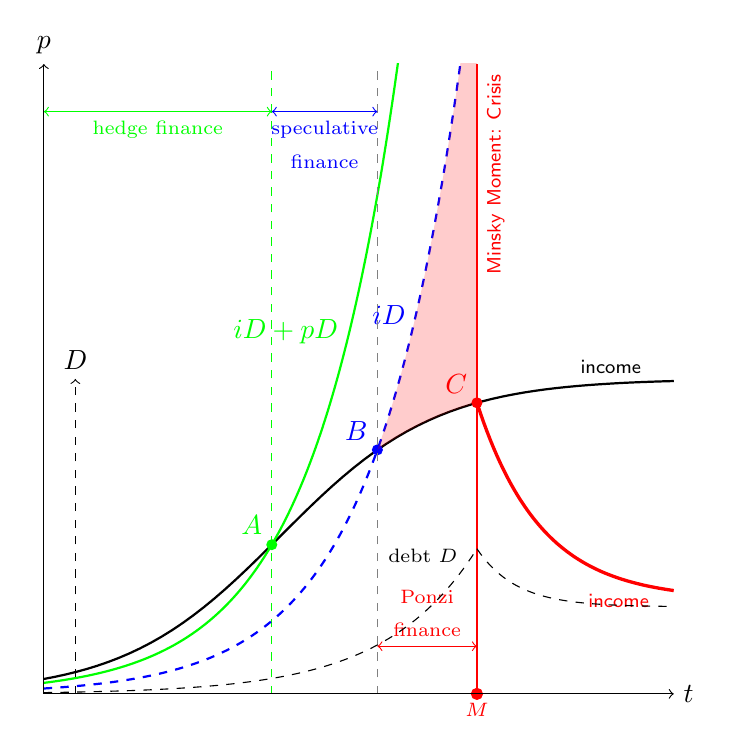
\begin{tikzpicture}[
    declare function={
        inc(\x)   = 4/(1+exp(-(\x-3)));                 % income: logistic
        intr(\x)  = 0.0685*exp(0.9*\x);                 % interest due
        serv(\x)  = 0.14*exp(0.9*\x);                   % interest + principal due
        crash(\x) = inc(\x) - 2.8*(1-exp(-1.2*(\x-5.5))); % income after the crash
        debt(\x)  = 0.01626*exp(0.86*\x);      
    },
    lbl/.style={font=\scriptsize, align=center,font=\sffamily},
    label at/.style 2 args={postaction={decorate, decoration={markings,mark=at position #1 with {\node[inner sep=2pt, anchor=south east] {#2};}}}},
]
    \coordinate (bot) at (0,0);
    \coordinate (top) at (0,8);
    \def\minsky{5.5}   % Minsky moment (set exogenously; see income after crash above)

    % --- invisible paths to find the phase boundaries ---
    \path[name path=inc]  plot[domain=0:6,    samples=150] (\x,{inc(\x)});
    \path[name path=serv] plot[domain=0:4.55, samples=150] (\x,{serv(\x)});
    \path[name path=intr] plot[domain=0:5.35, samples=150] (\x,{intr(\x)});
    \path[name intersections={of=inc and serv, by=A}]; % hedge -> speculative
    \path[name intersections={of=inc and intr, by=B}]; % speculative -> Ponzi
    % x-coordinate of B (in cm) for use as a plot domain
    \path (B); \pgfgetlastxy{\Bxpt}{\Bypt}
    \pgfmathsetmacro\Bx{\Bxpt/1cm}

        % crossing points
        \coordinate (C) at (\minsky,{inc(\minsky)});

    \begin{scope}
        \clip (0,-1em) rectangle (8,8);

        \draw[thick] plot[domain=0:8, samples=60] (\x,{inc(\x)});
        \node[lbl, above,font=\scriptsize\sffamily] at (7.2,{inc(7.2)}) {income};

        % curves
    
            
        \ifstep{1}{
            \begin{scope}[green]
            \draw[thick,label at={0.60}{$iD+pD$}]          plot[domain=0:4.55, samples=150] (\x,{serv(\x)});
            \fill (A) node[above left] {$A$} circle (2pt);
            % boundaries
            \draw[dashed] (A |- bot) -- (A |- top);
            % \node[font=\scriptsize\sffamily,anchor=north east,text width=12ex,align=center,rotate=45] at ($(A |- top) + (-2ex,-6ex)$) {Hedge Finance};
            \draw[<->] ($(0,|- top)+(0,-4ex)$) -- node[below] {\scriptsize hedge finance}  ($(A |- top)+(0,-4ex)$);
                    
            \end{scope}
        }

        \ifstep{2}{
            \begin{scope}[blue]
                \draw[ thick, dashed,label at={0.65}{$iD$}] plot[domain=0:5.35, samples=150] (\x,{intr(\x)}) node {interest};
                \fill (B) node[above left] {$B$} circle (2pt);
                \draw[gray, dashed] (B |- bot) -- (B |- top);
                \draw[<->] ($(A |- top)+(0,-4ex)$) -- node[below,text width=10ex,align=center] {\scriptsize speculative finance}  ($(B |- top)+(0,-4ex)$);
                
            \end{scope}
        }

    \ifstep{3}{ %%% Ponzi Finance, Minsky Momemnt
        \begin{scope}[red]
            \fill (C) node[above left] {$C$} circle (2pt);    
            % \draw[very thick]      plot[domain=0:\minsky, samples=150] (\x,{inc(\x)});
            \draw[very thick]      plot[domain=\minsky:8, samples=60] (\x,{crash(\x)});
            \draw[thick] (\minsky,0) -- (\minsky,8) node[below left,rotate=90,font=\scriptsize\sffamily] {Minsky Moment: Crisis};
            % Ponzi gap: starts exactly at B, shortfall covered only by new borrowing
            \fill[opacity=.2]
                plot[domain=\Bx:5.35, samples=60] (\x,{intr(\x)}) -- (\minsky,8.6)
                -- plot[domain=\minsky:\Bx, samples=60] (\x,{inc(\x)}) -- cycle;
            \filldraw (\minsky,0) node[below,font=\scriptsize]  {$M$} circle (2pt);
                \node[lbl, below,font=\scriptsize\sffamily] at (7.3,{crash(7.6)}) {income};
                % \node[font=\scriptsize\sffamily,rotate=45,anchor=south east,text width=6ex,align=center] at ($(C |- bot) + (0,+2cm)$) {Ponzi Finance};
                \draw[<->] ($(B |- bot)+(0,+4ex)$) -- node[above,text width=8ex,align=center] {\scriptsize Ponzi finance}  ($(C |- bot)+(0,+4ex)$);
                
        \end{scope}
    }

           
        
    \end{scope}


    % axes (drawn on top of the bands)
    \draw[->] (0,0)   -- (8,0) node[right] (Q) {$t$};
    \draw[->] (0,0)  -- (0,8) node[above] (P) {$p$};

    \ifstep{4}{% debt stock 
    
 
    \begin{scope}[dashed]%[yshift=-5.2cm]
        \coordinate (b2) at (0,0);
        \coordinate (t2) at (0,4);

        % \draw[gray, dashed] (A |- b2) -- (A |- t2);
        % \draw[gray, dashed] (B |- b2) -- (B |- t2);
        % \draw[red, thick] (\minsky,0) -- (\minsky,4);

        % debt keeps compounding until M, then defaults write part of it off
        \draw[label at={0.95}{\scriptsize debt $D$}]
            plot[domain=0:\minsky, samples=150] (\x,{debt(\x)});
            
            \draw plot[domain=\minsky:8, samples=60]
               (\x,{debt(\minsky)*(0.6+0.4*exp(-2*(\x-\minsky)))});
        % \node[lbl, above] at (7.2,{0.6*debt(\minsky)}) {debt overhang};

        % \draw[->] (0,0) -- (8,0) node[right] {$t$};
        \draw[->] (0.4,0) -- (0.4,4) node[above] {$D$};
        % \filldraw (\minsky,0) node[below,font=\scriptsize] {$M$} circle (2pt);
    \end{scope}

    }



\end{tikzpicture}
\end{document}